% Overleaf: compile with pdfLaTeX (the default compiler).
% Put this file at the Overleaf project root and upload the images/ folder beside it.
% From Docs/report/, the same figures are also found at ../../images/.
\documentclass[11pt]{article}

\usepackage[margin=1in]{geometry}
\usepackage{booktabs}
\usepackage{amsmath}
\usepackage{graphicx}
\graphicspath{{images/}{../../images/}}
\usepackage[font=small,skip=2pt]{caption}
\usepackage[hidelinks]{hyperref}

\newcommand{\placefig}[1]{%
  \par\vspace{0.4em}%
  \noindent\begin{minipage}{\textwidth}%
  \centering
  #1%
  \end{minipage}%
  \par\vspace{0.5em}%
}

\title{5228 progress report}
\date{September 2026}

\begin{document}
\maketitle

\section{Auxiliary features: construction, limits, and planned checks}
\label{sec:auxiliary}

The prediction target is \texttt{MONTHLY\_RENT}.
The rental row already has the approval month, town, block, street, flat type, flat model, floor area, furnished flag, lease year, and upfront fee.
The auxiliary files (blocks, MRT stations, schools, malls, COE prices, and stocks) do not share that row key.
Nothing below has been screened by correlation with rent, and no model has been trained.
The figures only describe the constructed columns.

\subsection{How the auxiliary tables meet the rental features}

The saved tables contain only the new columns, in source-row order, so the original rental fields are concatenated back at training time.
Stations, schools, and malls have coordinates but no block number.
The block table is the hub: it has both an address and coordinates, and every later spatial column starts from that join.

\paragraph{Block attributes and age.}
The rental row is left-joined to the block file on
\begin{equation}
\texttt{block\_key}
=
\mathrm{norm}(\texttt{BLOCK})
\mathbin{\Vert}
\mathrm{norm}(\texttt{STREET}),
\end{equation}
where \texttt{norm} strips, lowercases, and collapses spaces.
The key matches every training and test row, and the row count does not change.
The copied fields are latitude, longitude, postal code (\texttt{NIL} becomes null), maximum floor, year of completion, subzone, planning area, and region.
Building age is the approval year minus the completion year.
Lease age uses \texttt{LEASE\_COMMENCE\_DATE} instead.
A third column is the gap between those two years, and a product of building age with a Central Region flag lets a linear model treat age differently in the centre.
The motivation is that town alone does not say whether the block is central, new, or tall, and the same completion year is a different age in 2021 and in 2026.
Figure~\ref{fig:blocks} shows the joined region and those age and floor distributions.

\placefig{%
\begin{minipage}[t]{0.38\textwidth}
\centering
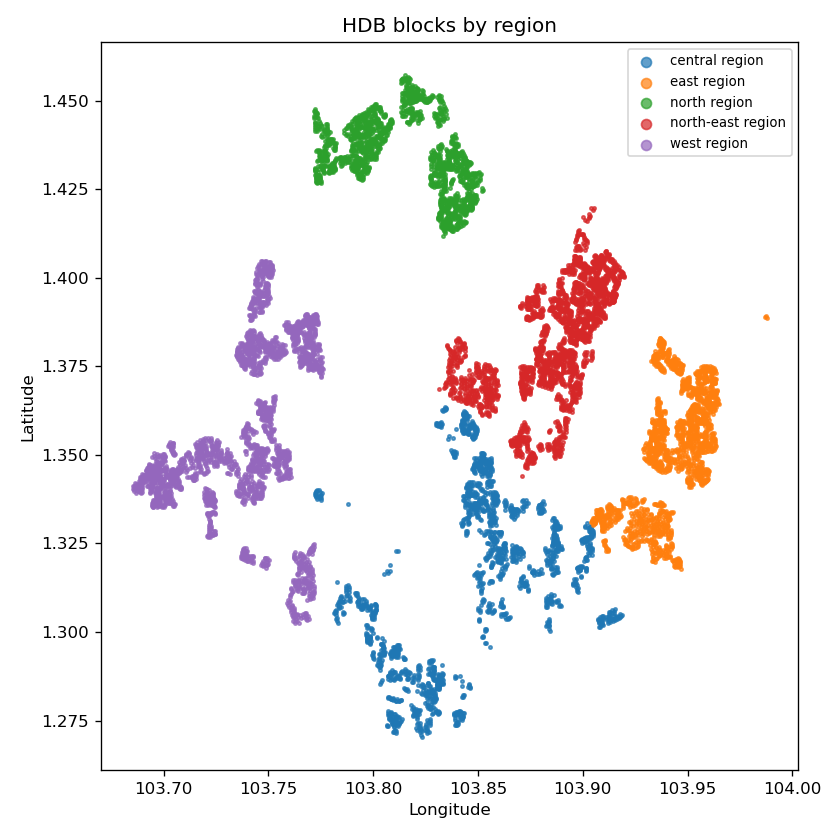
\includegraphics[width=\linewidth]{images/blocks_region_map.png}\\[0.2em]
{\small (a) Region after the address join.}
\end{minipage}\hfill
\begin{minipage}[t]{0.56\textwidth}
\centering
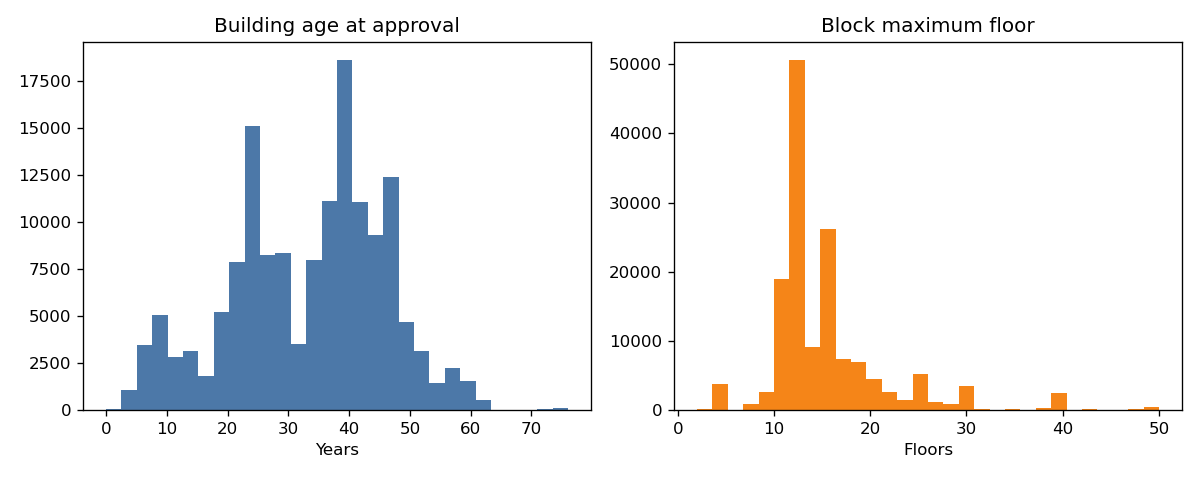
\includegraphics[width=\linewidth]{images/blocks_age_floor.png}\\[0.2em]
{\small (b) Age at approval, and maximum floor.}
\end{minipage}\\[0.35em]
\refstepcounter{figure}%
{\small Figure~\thefigure: Block attributes copied onto the rental rows.}%
\label{fig:blocks}%
}

\paragraph{MRT.}
Distances use Haversine with Earth radius 6{,}371\,km.
The open trunk set is stations with status \texttt{open} whose code prefix is NS, NE, CC, DT, TE, EW, or CG.
The two open Changi Airport (\texttt{CG}) stations are labelled EW.
For each block we store the nearest trunk station's distance, code, normalized name, and line, plus the nearest station and distance on each of the six lines, and the number of trunk codes within 0.5, 1, and 2\,km.
Ties closer than $10^{-6}$\,km keep the lexicographically smallest code.
Planned stations, and prefixes CR, JE, JS, JW, and CP, stay in their own distance columns so they cannot shrink the open-station distance.
A flag is 1 when the nearest trunk station's name has at least two codes.
The motivation is access: a flat near a station is easier to commute from, one distance cannot tell which corridor that station serves, and a count separates a single station from a cluster.
Figure~\ref{fig:mrt} shows that most rentals are within about 1\,km of some trunk station, that 0.5\,km is often empty, and that the North East Line is farther than the East--West Line.

\placefig{%
\begin{minipage}[t]{0.48\textwidth}
\centering
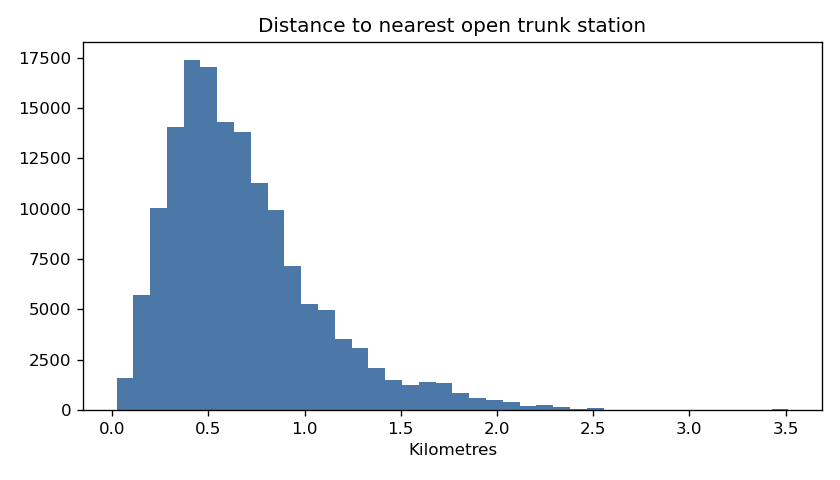
\includegraphics[width=\linewidth]{images/mrt_nearest_trunk.png}\\[0.2em]
{\small (a) Nearest open trunk station.}
\end{minipage}\hfill
\begin{minipage}[t]{0.48\textwidth}
\centering
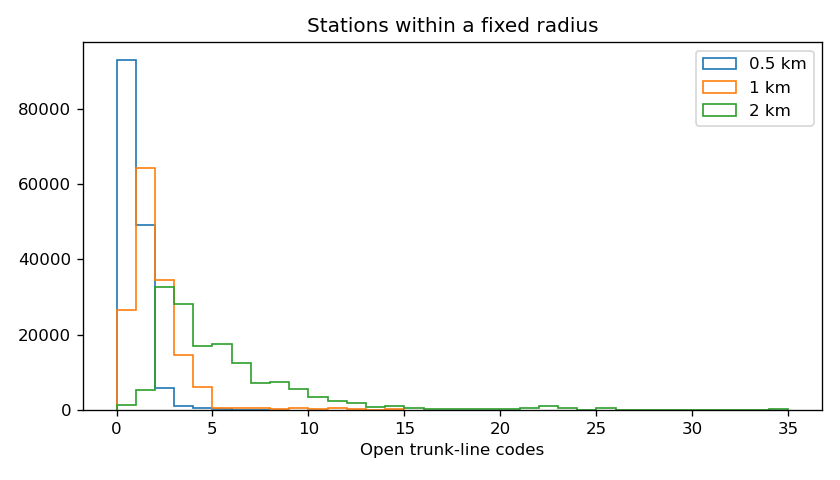
\includegraphics[width=\linewidth]{images/mrt_radius_counts.png}\\[0.2em]
{\small (b) Trunk-line codes within 0.5, 1, and 2\,km.}
\end{minipage}\\[0.45em]
\begin{minipage}[t]{0.58\textwidth}
\centering
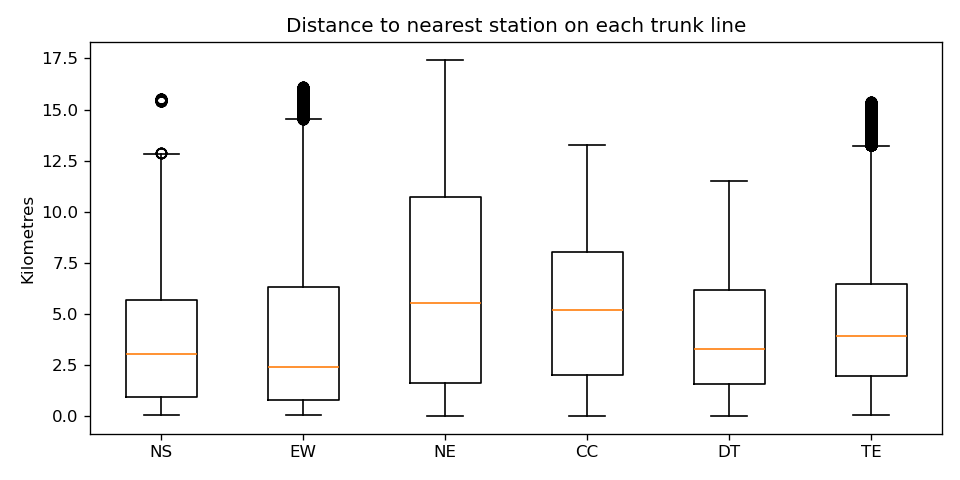
\includegraphics[width=\linewidth]{images/mrt_line_distances.png}\\[0.2em]
{\small (c) Nearest station on each trunk line.}
\end{minipage}\\[0.35em]
\refstepcounter{figure}%
{\small Figure~\thefigure: MRT access. An interchange is counted once per code.}%
\label{fig:mrt}%
}

\paragraph{Schools and malls.}
Primary schools are rows with \texttt{MAINLEVEL\_CODE} equal to \texttt{primary} (179 schools).
Secondary schools are the two strings \texttt{secondary (s1-s5)} and \texttt{secondary (s1-s4)} (133 schools).
Each set contributes a nearest distance, the normalized school name, and a count within 1\,km; primary schools also have a 2\,km count.
All 337 schools add one more nearest distance, name, and 1\,km count.
All 113 malls contribute the nearest distance, normalized name, and counts within 1 and 2\,km.
Names are kept because those tables have no code, and the normalized name is unique.
The motivation is daily convenience: households pay for a short walk to a primary school or a shop, and a count distinguishes one neighbour from several.
Figure~\ref{fig:amenity} shows schools packed closer than malls, and many rentals with no mall inside 1\,km.

\placefig{%
\begin{minipage}[t]{0.60\textwidth}
\centering
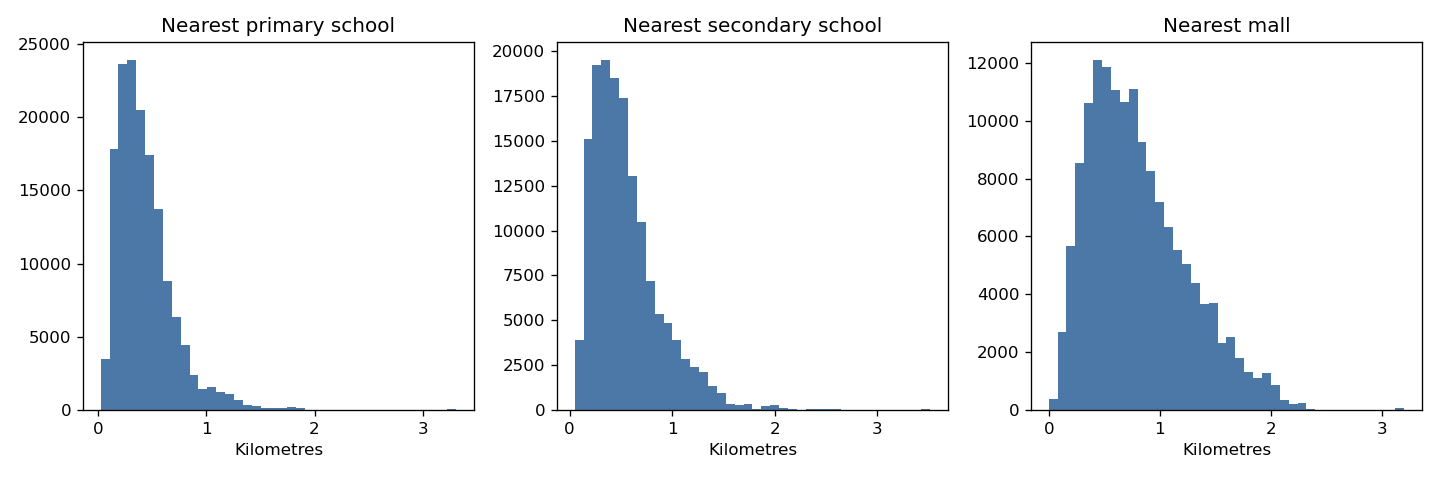
\includegraphics[width=\linewidth]{images/amenity_distances.png}\\[0.2em]
{\small (a) Nearest primary school, secondary school, and mall.}
\end{minipage}\hfill
\begin{minipage}[t]{0.36\textwidth}
\centering
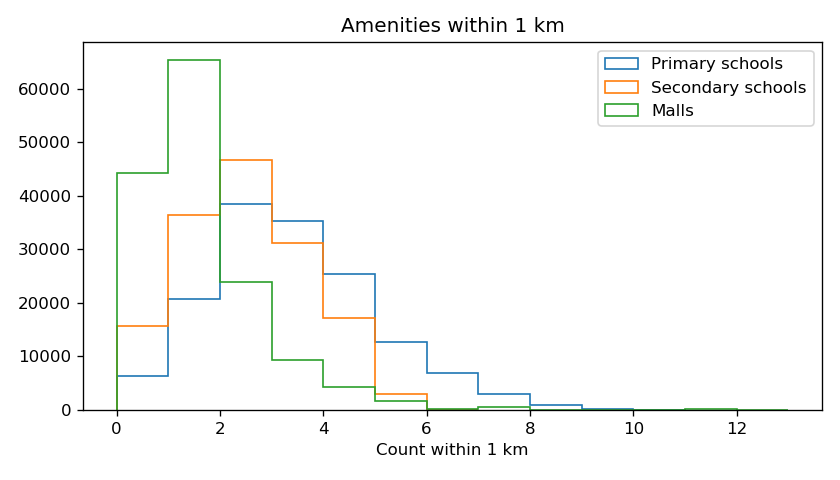
\includegraphics[width=\linewidth]{images/amenity_counts_1km.png}\\[0.2em]
{\small (b) Counts within 1\,km. Zero is a real zero.}
\end{minipage}\\[0.35em]
\refstepcounter{figure}%
{\small Figure~\thefigure: Schools and malls around the training rentals.}%
\label{fig:amenity}%
}

\paragraph{Density and a fixed downtown point.}
The number of other HDB blocks within 500\,m uses the same block coordinates, excluding the block itself.
The town centroid is the mean latitude and longitude of blocks in that town, and each block is measured to its own centroid.
Distance to the CBD is Haversine to the fixed Raffles Place coordinate $(1.283889, 103.851389)$, taken from station codes \texttt{ns26} and \texttt{ew14}.
A log of the nearest trunk distance, $\ln(d+0.001)$, gives nearby changes more weight than a linear model would give the raw kilometres.
The motivation is position inside a town and on the island: two flats in the same town can still sit at the edge or next to downtown.

\paragraph{COE and stocks.}
COE amounts are parsed by stripping dollar signs and commas.
Each category-month uses bidding round 2, or round 1 if round 2 is absent.
A rental in month $T$ receives the premium, the change from $T-2$ to $T-1$, and bids divided by quota, all from month $T-1$.
Categories A, B, and E have those three columns; category A also has the mean of $T-1$, $T-2$, and $T-3$; category C has only the lagged premium.
Stock features use month-end adjusted closes.
The bank basket is the equal-weight mean of \texttt{D05.SI}, \texttt{O39.SI}, and \texttt{U11.SI}; the property basket is \texttt{C09.SI}, \texttt{U14.SI}, and \texttt{9CI.SI}.
A month is used only when all three symbols have a close, and the rental again sees month $T-1$, both as a level and as that month's return.
The motivation is a market-wide shift that floor area and town cannot express: dearer car quotas or weaker bank shares may coincide with tighter household budgets.
Figure~\ref{fig:market} shows that both series are constant across flats approved in the same month.

\placefig{%
\begin{minipage}[t]{0.48\textwidth}
\centering
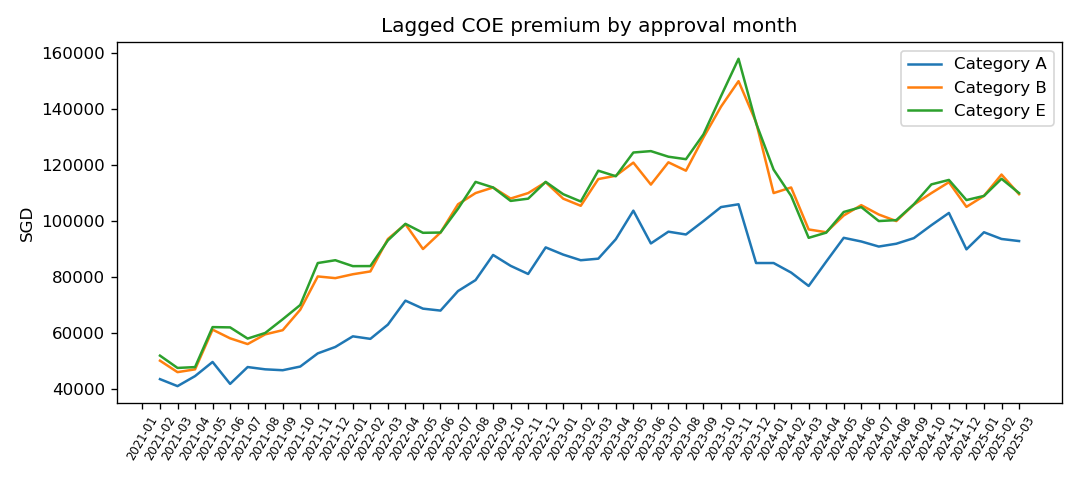
\includegraphics[width=\linewidth]{images/coe_monthly.png}\\[0.2em]
{\small (a) Lagged COE premium.}
\end{minipage}\hfill
\begin{minipage}[t]{0.48\textwidth}
\centering
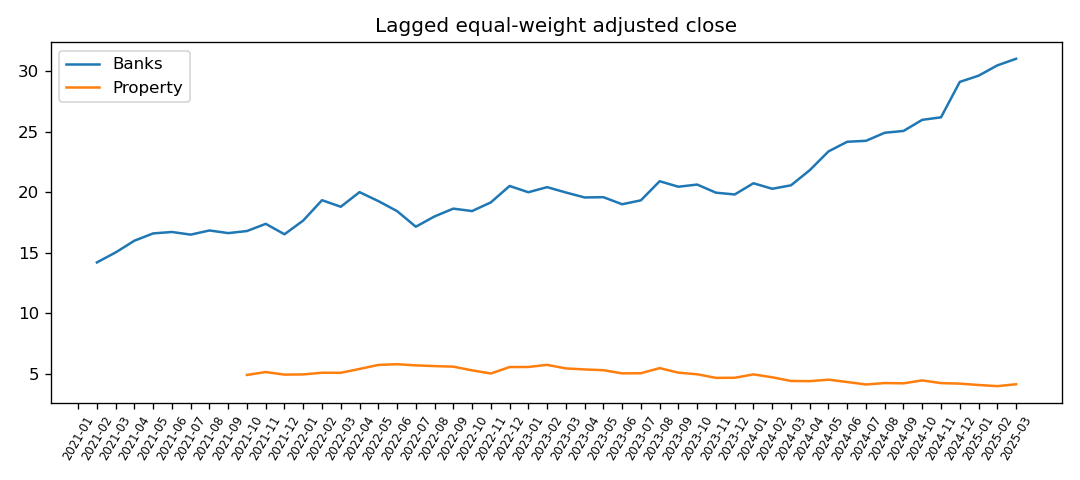
\includegraphics[width=\linewidth]{images/stock_baskets_monthly.png}\\[0.2em]
{\small (b) Lagged bank and property baskets.}
\end{minipage}\\[0.35em]
\refstepcounter{figure}%
{\small Figure~\thefigure: Month-level series shared by every flat approved in that month.}%
\label{fig:market}%
}

\paragraph{Group-mean rents.}
Six columns are target encodings.
For a row in month \(T\), only training rents from \(T-1\), \(T-2\), and \(T-3\) are used:
\begin{equation}
\frac{n\,\bar r_g + 20\,\bar r}{n + 20}.
\end{equation}
Here \(\bar r_g\) is the group mean inside that window, \(n\) is the number of those rows, and \(\bar r\) is the island-wide mean inside the same three months.
If \(n=0\), the value is \(\bar r\).
January 2021 has none of those months in the file, so all six columns are null.
February 2021 uses January only.
The groups are the first two digits of the postal code, the legacy district D01--D28 implied by those digits, \texttt{nearest\_mall\_name}, \texttt{nearest\_open\_mrt\_code}, \texttt{nearest\_primary\_name}, and \texttt{nearest\_secondary\_name}.
The sector and district strings are not stored.
The motivation is the recent local rent level: a mean accumulated since 2021 would still carry old rent levels into 2025, while the previous quarter moves with the market. Shrinkage keeps a thin quarter from being dominated by a few leases.
The month-by-group heatmaps in \texttt{outputs/figures/heatmap\_*.png} draw this formula even when that month has no rental in the group.
A cell is blank only when the three-month window contains no training rents.
The maps in \texttt{outputs/figures/maps/} place the same values on an OpenStreetMap background for each June and December whose window overlaps the training months.
Each land cell takes the colour of its single nearest mall, primary school, or open MRT station, and each map has its own colour scale.
Figure~\ref{fig:mrt-map} is the June 2025 MRT map.
Its window is March, April, and May 2025, and the training file ends in March 2025, so the colours use March 2025 rents only.
A darker patch is the service area of one station whose recent rents were higher. The scale belongs to this file alone.

\placefig{%
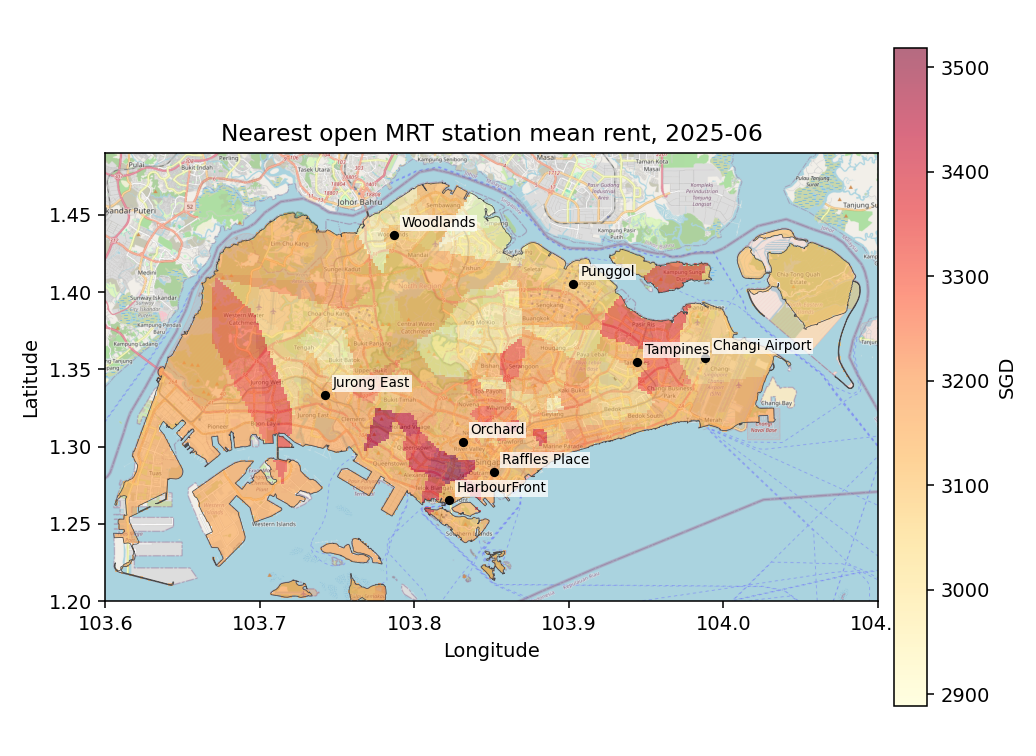
\includegraphics[width=0.92\linewidth]{../../outputs/figures/maps/map_mrt_2025-06.png}\\[0.35em]
\refstepcounter{figure}%
{\small Figure~\thefigure: Nearest open MRT station, June 2025. Colour is the smoothed mean of training rents in the previous three months for that station. Each area is one station.}%
\label{fig:mrt-map}%
}

\subsection{Limits of the built columns}

\begin{itemize}
\item \texttt{MAX\_FLOOR} is the top floor of the block. Values of $-1$ on floor and completion year are sentinels and are stored as null (159 training rows, no test rows).
\item The MRT file has no opening date. A station marked open may have opened after January 2021. Planned stations and future-line prefixes are kept out of the open-station distance.
\item About 20 MRT longitudes have only one to three decimal places. Switching from Haversine to SVY21 does not repair that.
\item Great-circle distance is not walking time. School and mall tables have no opening dates, and the school table has no university.
\item COE and stock columns are constant within an approval month. January 2021 COE lags are null because December 2020 is missing. The property basket is missing on early training rows because one constituent starts later.
\item Group means are target encodings of the previous three months of rents, not properties of a mall, station, or school. January 2021 is null. A mall mean covers rentals for which that mall is the nearest mall, not every flat inside a radius.
\item Empty postal codes (285 blocks) have no postal-sector group and fall back to that quarter's island-wide mean once the three-month window contains any training rent.
\end{itemize}

\subsection{How the features will be tested}

This check has not been run.
Train on earlier approval months and validate on later months, and use that same split for every model.
Do not fit group means, or any other rent statistic, on the validation months.

Start with the mean training rent, then a linear model on the original rental fields only.
Add one auxiliary family at a time: block and age, MRT, schools and malls, density and CBD distance, COE and stocks, then group-mean rents.
Repeat the same feature sets with XGBoost and a multilayer perceptron.
Trees can split raw distances and categories; the linear model and the MLP depend more on scaling and on the explicit transforms.
Use family ablation for groups of columns, and linear coefficients or permutation importance for single columns.
A column is kept only if it lowers validation RMSE under this split.
An in-sample correlation with rent is not enough, especially for the group means, which repeat recent rents unless the time split is enforced.

\end{document}
